\documentclass[a4paper, 12pt]{report}

%====================== PACKAGES ======================

\usepackage[french]{babel}
\usepackage[utf8x]{inputenc}
%pour gérer les positionnement d'images
\usepackage{float}
\usepackage{amsmath}
\usepackage{graphicx}
\usepackage[colorinlistoftodos]{todonotes}
\usepackage{url}
%pour les informations sur un document compilé en PDF et les liens externes / internes
\usepackage{hyperref}
%pour la mise en page des tableaux
\usepackage{array}
\usepackage{tabularx}
%pour utiliser \floatbarrier
%\usepackage{placeins}
%\usepackage{floatrow}
%espacement entre les lignes
\usepackage{setspace}
%modifier la mise en page de l'abstract
\usepackage{abstract}
%police et mise en page (marges) du document
\usepackage[T1]{fontenc}
\usepackage[top=2cm, bottom=2cm, left=2cm, right=2cm]{geometry}
%Pour les galerie d'images
\usepackage{subfig}
\usepackage{eurosym}
%Pour la mise en page du code
\usepackage{listings}
\usepackage{color}
\definecolor{dkgreen}{rgb}{0,0.6,0}
\definecolor{gray}{rgb}{0.5,0.5,0.5}
\definecolor{mauve}{rgb}{0.58,0,0.82}



\lstdefinestyle{tf}{frame=shadowbox,
	rulesepcolor=\color{gray},
	framexleftmargin=5mm,
	aboveskip=3mm,
	belowskip=3mm,
	showstringspaces=false,
	columns=flexible,
	basicstyle={\small\ttfamily},
	numbers=left,
	numberstyle=\tiny,
	breaklines=true,
<<<<<<< HEAD
	breakatwhitespace=false,
=======
	breakatwhitespace=true,
>>>>>>> 6e0e4c269c4e06128cc702a8f257ca79eca8d33b
	tabsize=3
}

\lstset{frame=tb,
	rulesepcolor=\color{gray},
	framexleftmargin=5mm,
	language=bash,
	aboveskip=3mm,
	belowskip=3mm,
	showstringspaces=false,
	columns=flexible,
	basicstyle={\small\ttfamily},
	numbers=left,
	numberstyle=\tiny,
	keywordstyle=\color{blue},
	stringstyle=\color{mauve},
	breaklines=true,
<<<<<<< HEAD
	breakatwhitespace=false,
	literate={;}{{;\allowbreak}}1,
=======
	breakatwhitespace=true,
>>>>>>> 6e0e4c269c4e06128cc702a8f257ca79eca8d33b
	tabsize=3
}

%====================== INFORMATION ET REGLES ======================

%rajouter les numérotation pour les \paragraphe et \subparagraphe
\setcounter{secnumdepth}{4}
\setcounter{tocdepth}{4}

\hypersetup{							% Information sur le document
pdfauthor = {Sugdenaz EKICI,
			Yahia KHERZA,
			Olivier MARAVAL,
    		Valentin VIRET-JACQUOT},			% Auteurs
pdftitle = {Architecture logicielle et notice d'installation / utilisation du poste de développement},			% Titre du document
pdfsubject = {Mémoire de Projet},		% Sujet
pdfkeywords = {Tag1, Tag2, Tag3, ...},	% Mots-clefs
pdfstartview={FitH}}					% ajuste la page à la largueur de l'écran
%pdfcreator = {MikTeX},% Logiciel qui a crée le document
%pdfproducer = {}} % Société avec produit le logiciel

%======================== DEBUT DU DOCUMENT ========================

\begin{document}

\addtocontents{toc}{\protect\thispagestyle{empty}}

%régler l'espacement entre les lignes
\newcommand{\HRule}{\rule{\linewidth}{0.5mm}}

%page de garde
\begin{titlepage}
\begin{center}

% Upper part of the page. The '~' is needed because only works if a paragraph has started.
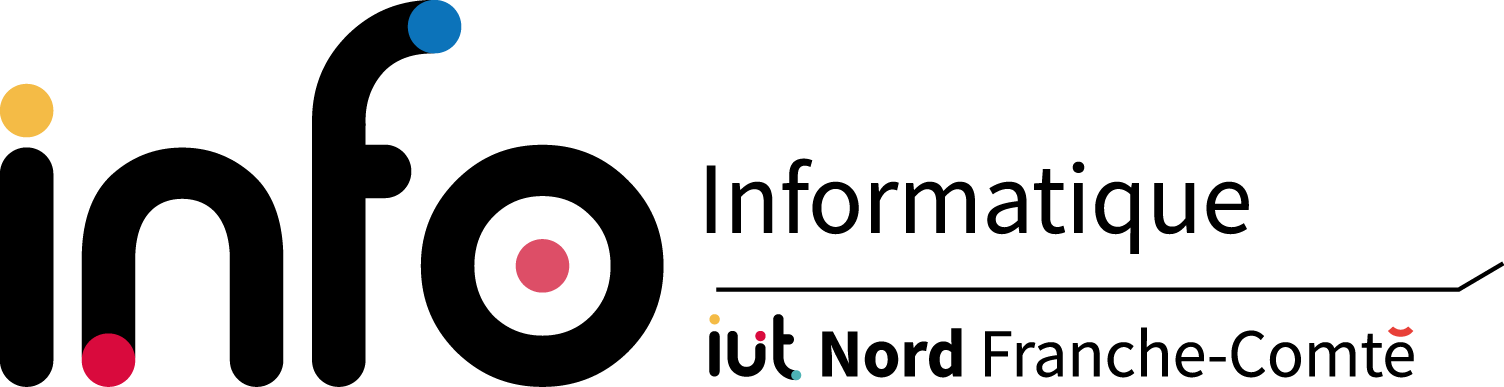
\includegraphics[width=0.5\textwidth]{./images/InfoLogoQuadriH.png}~\\[1cm]

\textsc{\LARGE SAE 1.03 - BUT INFORMATIQUE - GROUPE 1}\\[1.5cm]

\textsc{\Large }\\[0.5cm]

% Title
\HRule \\[0.4cm]

{\huge \bfseries Architecture logicielle et notice d'installation / utilisation du poste de développement\\[0.4cm] }

\HRule \\[1.5cm]

% Author and supervisor
\begin{minipage}{0.4\textwidth}
\begin{flushleft} \large
\emph{Auteur:}\\
Sugdenaz \textsc{Ekici}(\textit{A1})\\
Yahia \textsc{Kherza}(\textit{A1})\\
Olivier \textsc{Maraval}(\textit{A1})\\
Valentin \textsc{Viret-Jacquot}(\textit{A1})
\end{flushleft}
\end{minipage}
\begin{minipage}{0.4\textwidth}
\begin{flushright} \large
\emph{Client:} \\
Michel \textsc{Salomon}\\
\emph{Référent:} \\
Olivier \textsc{Maraval}
\end{flushright}
\end{minipage}

\vfill

% Bottom of the page
{\large \today}

\end{center}
\end{titlepage}

%page blanche
\newpage
~
\thispagestyle{empty}

\pagenumbering{gobble}
\tableofcontents
\thispagestyle{empty}

%ne pas numéroter le sommaire

\newpage

%espacement entre les lignes d'un tableau
\renewcommand{\arraystretch}{1.5}

%====================== INCLUSION DES PARTIES ======================

~
\thispagestyle{empty}


\newpage
\pagenumbering{arabic}

\setcounter{page}{5}

\chapter{Installation du Système de Base}

\section{Accéder au programme d'installation}

Si votre pc démarre directement sur le programme d'installation, vous pouvez vous rendre directement à la section suivante.

\begin{itemize}
\item Connectez la clé USB bootable fournit à votre ordinateur. Cette dernière contient l'ISO Débian suivant : \textit{\href{https://cdimage.debian.org/debian-cd/current/amd64/iso-dvd/debian-12.2.0-amd64-DVD-1.iso}{debian-12.2.0-amd64-DVD-1.iso}}
\item Démarrez votre ordinateur et accédez au menu de démarrage du BIOS en appuyant sur la touche appropriée (généralement F2, F10, F12 ou Suppr) au démarrage de l'ordinateur.
\item Sélectionnez la clé USB comme périphérique de démarrage et appuyez sur Entrée pour démarrer votre ordinateur à partir de la clé USB.\\
\end{itemize}

Vous vous déplacerez dans le menu d'installation avec les \textbf{Touches Fléchées}. La touche \textbf{Espace} sélectionne une option et la touche \textbf{Entrée} valide un choix.\\

Vous serez accueilli par un écran d'installation vous indiquant plusieurs options.

\section{Ecran d'installation}
\begin{itemize}
	\item Sélectionnez la deuxième option : \textbf{Install}
\end{itemize}

\section{Select a language}
\begin{itemize}
	\item Choisissez \textbf{French - Français} dans la liste et appuyez sur \textbf{Entrée}
\end{itemize}

\section{Choix de votre situation géographique}
\begin{itemize}
	\item Choisissez \textbf{France} dans la liste et appuyez sur \textbf{Entrée}
\end{itemize}

\section{Configurer le clavier}
\begin{itemize}
	\item Choisissez \textbf{Français} dans la liste
\end{itemize}

\section{Configurer le réseau}

\begin{itemize}
	\item Dans le champ \textbf{Nom de machine} inscrivez le texte : \texttt{poste-dev-1}
	\item Laissez le champ \textbf{Domaine} vide
\end{itemize}

\section{Créer les utilisateurs et choisir les mots de passe}
\begin{itemize}
	\item Dans le champ \textbf{Mot de passe du superutilisateur (" root ")} écrivez : \texttt{\$sae3*2023\$}
	\item Réécrivez le même mot de passe dans le champ \textbf{Confirmation du mot de passe}
	\item Dans le champ \textbf{Nom complet du nouvel utilisateur} entrez : \texttt{Michel Salomon}
	\item Dans le champ \textbf{Identifiant pour le compte utilisateur} entrez : \texttt{msalomon}
	\item Dans le champ \textbf{Mot de passe pour le nouvel utilisateur} entrez : \texttt{CqriT}
	\item Réécrivez le même mot de passe dans le champ \textbf{Confirmation du mot de passe}
\end{itemize}

\section{Partitionner les disques}
\begin{itemize}
	\item Dans la liste \textbf{Méthode de partionnement} sélectionnez la dernière option : \textbf{Manuel}
	\item Sélectionnez dans la liste le disque sur lequel vous souhaitez installer Debian.
	\item Répondez \textbf{Oui} à la question : \textit{"Faut-il créer une nouvelle table des partitions sur ce disque ?"}
\end{itemize}

\section{Partition /}
	\begin{itemize}
	\item Sélectionnez la nouvelle option venant d'apparaître sur la liste et terminant par \textbf{"Espace libre"}
		\begin{itemize}
			\item Sélectionnez \textbf{Créer une nouvelle partition}
			\item Dans le champ \textbf{Nouvelle taille de la partition} entrez la valeur : \texttt{10 GB}
			\item Dans la liste \textbf{Type de la nouvelle partition} sélectionnez : \textbf{Primaire}
			\item Dans la liste \textbf{Emplacement de la nouvelle partition} sélectionnez : \textbf{Début}
			\item Dans la liste \textbf{Caractéristiques de la partition} sélectionnez : \textbf{Fin du paramétrage de cette partition}\\	
		\end{itemize}
	\end{itemize}
La nouvelle partition a du apparaitre en n°1 dans la liste.
		
\subsection{Partition swap}
	\begin{itemize}
		\item Sélectionnez de nouveau l'option terminant par \textbf{"Espace libre"}
		\begin{itemize}
			\item Sélectionnez \textbf{Créer une nouvelle partition}
			\item Dans le champ \textbf{Nouvelle taille de la partition} entrez la valeur : \texttt{2 GB}
			\item Dans la liste \textbf{Type de la nouvelle partition} sélectionnez : \textbf{Logique}
			\item Dans la liste \textbf{Emplacement de la nouvelle partition} sélectionnez : \textbf{Début}
			\item Dans la liste \textbf{Caractéristiques de la partition} sélectionnez : \textbf{Utiliser comme} et choisissez : \textbf{espace d'échange ("swap")} dans la liste qui vient d'apparaitre.
			\item De retour dans la liste \textbf{Caractéristiques de la partition} sélectionnez : \textbf{Fin du paramétrage de cette partition}
		\end{itemize}	
	\end{itemize}
	
\subsection{Partition /opt}
\begin{itemize}
	\item Sélectionnez de nouveau l'option terminant par \textbf{"Espace libre"}
	\begin{itemize}
		\item Sélectionnez \textbf{Créer une nouvelle partition}
		\item Dans le champ \textbf{Nouvelle taille de la partition} entrez la valeur : \texttt{10 GB}
		\item Dans la liste \textbf{Type de la nouvelle partition} sélectionnez : \textbf{Logique}
		\item Dans la liste \textbf{Emplacement de la nouvelle partition} sélectionnez : \textbf{Début}
		\item Dans la liste \textbf{Caractéristiques de la partition} sélectionnez : \textbf{Point de montage} et choisissez : \textbf{/opt} dans la liste qui vient d'apparaitre.
		\item De retour dans la liste \textbf{Caractéristiques de la partition} sélectionnez : \textbf{Fin du paramétrage de cette partition}
	\end{itemize}	
\end{itemize}

\subsection{Partition /home}
\begin{itemize}
	\item Sélectionnez de nouveau l'option terminant par \textbf{"Espace libre"}
	\begin{itemize}
		\item Sélectionnez \textbf{Créer une nouvelle partition}
		\item Dans le champ \textbf{Nouvelle taille de la partition} entrez la valeur : \texttt{100\%}
		\item Dans la liste \textbf{Type de la nouvelle partition} sélectionnez : \textbf{Logique}
		\item Dans la liste \textbf{Emplacement de la nouvelle partition} sélectionnez : \textbf{Début}
		\item Dans la liste \textbf{Caractéristiques de la partition} sélectionnez : \textbf{Point de montage} et choisissez : \textbf{/home} dans la liste qui vient d'apparaitre.
		\item De retour dans la liste \textbf{Caractéristiques de la partition} sélectionnez : \textbf{Fin du paramétrage de cette partition}
	\end{itemize}	
\end{itemize}



\subsection{Finalisation des partitions}
\begin{itemize}
	\item Sélectionnez l'option \textbf{"Terminer le partitionnement et appliquer les changements"}
	\item Répondez \textbf{Oui} à la question : \textit{Faut-il appliquer les changements sur les disques ?}\\
\end{itemize}

L'installation du système de base va alors commencer, vous pourrez suivre son avancement grâce à la barre de chargement. Ce processus durera plus ou moins longtemps selon les caractéristiques de votre machine.

\section{Configurer l'outil de gestion des paquets}
\begin{itemize}
	\item Répondre \textbf{Non} à la question : \textit{Faut-il analyser d'autres supports d'installation ?}
	\item Répondre \textbf{Oui} à la question : \textit{Faut-il utiliser un miroir sur le réseau ?}
	\item Dans la liste \textbf{Pays du miroir de l'archive Debian} sélectionnez : \textbf{France}
	\item Dans la liste \textbf{Miroir de l'archive Debian} sélectionnez : \textbf{ftp.fr.debian.org}
	\item Laissez le champ \textbf{Mandataire HTTP} vide
	\item Répondre \textbf{Non} à la question : \textit{Souhaitez-vous participer à l'étude statistique sur l'utilisation des paquets ?}
\end{itemize}

\section{Sélection des logiciels}
\begin{itemize}
	\item Décochez les logiciels sélectionnés par défaut dans la liste \textbf{Logiciels à installer} en utilisant la \textbf{Barre espace}
	\item De la même façon, cochez les logiciels : \textbf{serveur SSH} et \textbf{utilitaires usuels du système} (seules ces deux cases doivent être cochées)
	\item Une fois la sélection effectuée vous pouvez valider avec \textbf{Entrée}
\end{itemize}

\section{Configuration de grub-pc}
\begin{itemize}
	\item Répondre \textbf{Oui} à la question : \textit{"Installer le programme de démarrage GRUB sur le disque principal}
	\item Dans la liste \textbf{Périphérique où sera installé le programme de démarrage} sélectionnez l'option indiquant le disque que vous venez de partitionner.
\end{itemize}

\section{Terminer l'installation}
Si le message \textbf{Installation terminée} s'affiche vous pouvez sélectionner l'option \textbf{Continuer} qui redémarrera l'ordinateur. Pensez à retirer le support d'installation et vous devriez vous retrouver face à un terminal affichant un curseur clignotant juste après le texte : \texttt{poste-dev-1 login:}
\chapter{Configuration en mode texte}

\section{Pré-requis}
Connectez vous avec le compte root en utilisant les informations suivantes :
\begin{itemize}
	\item \textbf{login :} \texttt{root}
	\item \textbf{Password :} \texttt{\$sae3*2023\$}
\end{itemize}

\section{Ajouter les dépôts supplémentaires}
Ouvrez le fichier \textbf{sources.list} à l'aide d'un éditeur de texte. Par exemple, vous pouvez utiliser la commande suivante pour ouvrir le fichier avec l'éditeur de texte \texttt{nano} :
\begin{lstlisting}
	nano /etc/apt/sources.list
\end{lstlisting}

Dans le fichier \textbf{sources.list}, vous verrez des lignes commençant par \textbf{"deb"} suivies d'une URL. Ces lignes représentent les dépôts principaux (main). Pour ajouter les dépôts \textbf{"contrib"} et \textbf{"non-free"}, vous devez les ajouter à la fin de chaque ligne correspondante.

Vous pouvez aussi commenter la première ligne en y ajoutant \texttt{\#} ou la supprimer si vous ne souhaitez pas utiliser les paquets du DVD (qui sont inutiles si vous avez une connexion internet)\\

Votre fichier devrait avoir les lignes suivantes
\begin{lstlisting}[style=tf]
deb http://ftp.fr.debian.org/debian bookworm main non-free-firmware contrib non-free
deb-src http://ftp.fr.debian.org/debian bookworm non-free-firmware main contrib non-free

deb http://ftp.fr.debian.org/debian-security/ bookworm-security main non-free-firmware contrib non-free
deb-src http://ftp.fr.debian.org/debian-security/ bookworm-security main non-free-firmware contrib non-free

deb http://ftp.fr.debian.org/debian bookworm-updates main non-free-firmware contrib non-free
deb-src http://ftp.fr.debian.org/debian bookworm-updates main non-free-firmware contrib non-free
\end{lstlisting}

Enfin, avec \texttt{nano}, vous pouvez valider vos modification en appuyant sur les touches \textbf{CTRL + O} puis \textbf{Entrée} et enfin \textbf{CTRL+X}

Vous pouvez maintenant mettre à jour la liste de paquets en utilisant la commande suivante :

\begin{lstlisting}
apt update
\end{lstlisting}

\section{Installer le support souris en mode texte}

Utilisez la commande suivante pour installer le paquet \texttt{gpm}, qui fournit le support de la souris dans le shell :

\begin{lstlisting}
apt install -y gpm
\end{lstlisting}

Maintenant, vous pouvez utiliser \texttt{gpm} pour sélectionner, copier et coller du texte dans une console. Voici quelques commandes utiles :
\begin{itemize}
\item \textbf{Pour sélectionner du texte :} Maintenez le \textbf{bouton gauche} de la souris enfoncé et faites glisser la souris sur le texte que vous souhaitez sélectionner.
\item \textbf{Pour copier et coller le texte sélectionné :} Appuyez sur le \textbf{bouton du milieu} pour copier le texte sélectionné dans le presse-papiers.
\item \textbf{Pour étendre la sélection :} Appuyez sur le \textbf{bouton droit} de la souris pour sélectionner le texte jusqu'au prochain espace. Vous pouvez aussi effectuer un \textbf{double-clic} pour le même effet.
\item \textbf{Pour sélectionner la ligne entière :} Effectuez un \textbf{triple-clic} pour sélectionner l'entièreté d'une ligne.
\end{itemize}

\section{Modification du groupe staff}

Exécutez la commande suivante pour modifier le groupe \texttt{staff} et lui donner le \texttt{gid} 500

\begin{lstlisting}
groupmod -g 500 staff
\end{lstlisting}

\section{Modification de l'utilisateur msalomon}

Executez les commandes suivantes pour assigner l'utilisateur aux groupes \texttt{staff} (qui sera son groupe principal) et au groupe \texttt{adm} puis enregistrer les informations suivantes :
\begin{itemize}
	\item \textbf{Full name} = Michel Salomon
	\item \textbf{Room} = E004
	\item \textbf{Work phone} = 03.84.58.77.76
\end{itemize}
La dernière commande supprimera le groupe au nom de l'utilisateur.

\begin{lstlisting}
usermod -u 2500 -g 500 -G adm msalomon
chfn -f "Michel Salomon" -r "E004" -w "03.84.58.77.76" msalomon
groupdel msalomon
\end{lstlisting}

\section{Ajout de l'utilisateur visiteur}
Créez d'abord le groupe \texttt{external} avec le gid 1000 :
\begin{lstlisting}
groupadd -g 1000 external
\end{lstlisting}

Ensuite, créez l'utilisateur \texttt{visiteur} avec le uid 3000 et le gid 1000 :
\begin{lstlisting}
useradd -u 3000 -g 1000 -M -N -s /usr/sbin/nologin visiteur
\end{lstlisting}
\emph{Note : Les options -M et -N sont utilisées pour ne pas créer de répertoire personnel et ne pas créer de groupe pour l'utilisateur, respectivement.}\\

Enfin, définissez le mot de passe pour l'utilisateur \texttt{visiteur} :
\begin{lstlisting}
echo 'visiteur:CqriT' | chpasswd
\end{lstlisting}

\section{Création des clés SSH pour msalomon}

On va générer pour l'utilisateur \texttt{msalomon}
\begin{itemize}
\item une paire de clés ED25519
\item une paire de clés RSA de 4096 bits
\end{itemize}

Passez à l'utilisateur \texttt{msalomon}. Pour cela, utilisez la commande suivante :

\begin{lstlisting}
su - msalomon
\end{lstlisting}

Créez une paire de clés ED25519 en utilisant la commande \texttt{ssh-keygen} suivante. Lorsqu'il vous sera demandé d'entrer une passphrase, tapez \texttt{azerty}.
\begin{lstlisting}
ssh-keygen -t ed25519 -f ~/.ssh/id_ed25519
\end{lstlisting}

Répétez l'opération pour la paire de clés RSA de 4096 bits :
\begin{lstlisting}
ssh-keygen -t rsa -b 4096 -f ~/.ssh/id_rsa
\end{lstlisting}

Vous aurez alors deux paires de clés SSH protégées par la passphrase \texttt{azerty} dans le répertoire \texttt{~/.ssh} de l'utilisateur \texttt{msalomon}

Vous pouvez maintenant revenir au compte \texttt{root} en tapant \texttt{exit} dans le terminal
\chapter{Configuration réseau}
<<<<<<< HEAD

\section{Adresse IP de la machine virtuelle et de l'hôte}

\subsection{IP de la machine virtuelle}

Vous pouvez accéder à l'adresse IP de la machine virtuelle en utilisant la commande suivante :

\begin{lstlisting}
ip addr show
\end{lstlisting}

Vous devriez avoir deux sections, celle qui vous intéresse est celle qui ne commence pas par \texttt{lo: <LOOPBACK}...

Dans la section pertinente, votre adresse ip se trouve à droite du mot \texttt{inet}\\

exemple : 
\begin{lstlisting}[style=tf]
inet 10.0.2.15/24 brd 10.0.2.255 scope global dynamicenp0s3
\end{lstlisting}
ici, l'ip est \texttt{10.0.2.15}

\subsection{IP de la machine hôte}
Vous pouvez utiliser la commande suivante pour afficher la table de routage :
\begin{lstlisting}
ip route
\end{lstlisting}
Cette dernière vous donnera plusieurs valeurs et il est possible de déduire laquelle correspond à l'adresse ip de la machine hôte :
\begin{lstlisting}[style=tf]
default via 10.0.2.2 dev enp0s3
10.0.2.0/24 dev enp0s3 proto kernel scope link src 10.0.2.15
169.254.0.0/16 dev enp0s3 scope link metric 1000
\end{lstlisting}
ici on peut déduire que l'adresse ip de la machine hôte est \texttt{10.0.2.2}.\\

\section{Fichier de configuration pour SSH}

Passez à l'utilisateur \texttt{msalomon}. Pour cela, utilisez la commande suivante :

\begin{lstlisting}
su - msalomon
\end{lstlisting}

Réduisez l'accès au répertoire \textit{.ssh} en modifiant les droits d'accès avec la commande :

\begin{lstlisting}
chmod 700 ~/.ssh
\end{lstlisting}

Créez un fichier de configuration dans le dossier \texttt{.ssh}, réduisez les droits d'accès au seul propriétaire et ouvrez-le pour modification grâce aux commandes suivantes :
\begin{lstlisting}
touch ~/.ssh/config
chmod 600 ~/.ssh/config
nano .ssh/config
\end{lstlisting}

Écrire les informations suivantes dans le fichier qui vient de s'ouvrir et l'enregistrer

\begin{lstlisting}[style=tf]
Host machineHote
	Hostname 10.0.2.2
	User userHote
	IdentityFile ~/.ssh/id_rsa
\end{lstlisting}

Enfin, vous pourrez copier la clé publique de la paire rsa dans le compte utilisateur sur la vraie machine via la commande suivante :

\begin{lstlisting}
ssh-copy-id -i ~/.ssh/id_rsa.pub machineHote
\end{lstlisting}

=======
>>>>>>> 6e0e4c269c4e06128cc702a8f257ca79eca8d33b

<<<<<<< HEAD
\chapter{Répertoire partagé}

\section{Récupération des Guest Additions}

Récupérer l'image iso des Guest Additions au niveau de \href{https://download.virtualbox.org/virtualbox/}{https://download.virtualbox.org/virtualbox/}, vous pouvez utiliser le lien ci-dessous en remplaçant le mot \texttt{VERSION} par votre numéro de version

\begin{lstlisting}
	https://download.virtualbox.org/virtualbox/VERSION/VBoxGuestAdditions_VERSION.iso
\end{lstlisting}

Démarrer la machine virtuelle et se connecter en super-utilisateur, puis faire les manipulations qui suivent pour insérer l'ISO dans le lecteur virtuel de la machine virtuelle :
\begin{itemize}
	\item Rendez-vous sur l'écran contenant votre VM lancée
	\item Périphériques > Lecteurs Optiques > Choose a disk file...
	\item Sélectionnez l'ISO que vous avez téléchargé.
\end{itemize}

\section{Installation de l'ISO}

Créer le répertoire qui doit servir de point de montage s'il n'existe pas déjà

\begin{lstlisting}
	mkdir /media/cdrom
\end{lstlisting}

Exécutez les commandes suivantes pour monter le CD dans ce répertoire, installer le nécessaire pour l'installation du contenu du disque et enfin lancer l'installateur présent sur ce disque.

\begin{lstlisting}
	mount -t iso9660 /dev/cdrom /media/cdrom
	apt update
	apt install -y build-essential linux-headers-`uname -r`
	cd /media/cdrom
	./VBoxLinuxAdditions.run
\end{lstlisting}

Redémarrer votre machine virtuelle à la fin de l'installation

\section{Vérification}

Reconnectez-vous en super-utilisateur et confirmez qu'il puisse accéder au répertoire partagé en Lecture/Écriture grâce à la commande suivante :

\begin{lstlisting}
	ls -l / |grep localhome|cut -d " " -f 1
\end{lstlisting}

À partir de la deuxième lettre de la chaine de caractère qui apparaît, vous devez avoir, au minimum, rw (normalement rwx).\\

On va maintenant permettre à l'utilisateur msalomon d'avoir les droits en lecture et en écriture sur le dossier en l'ajoutant au groupe vboxsf:

\begin{lstlisting}
	usermod -aG vboxsf msalomon
\end{lstlisting}

=======
\chapter{Répertoire partagé}
>>>>>>> 6e0e4c269c4e06128cc702a8f257ca79eca8d33b

\chapter{Environnement de bureau}

\section{Installation de la commande sudo}

Puisqu'il est déconseillé de se connecter à l'environnement de bureau en tant que super-utilisateur, nous allons commencer par installer la commande \texttt{sudo} :

\begin{lstlisting}
apt install sudo
\end{lstlisting}

Nous allons maintenant ajouter l'utilisateur \texttt{msalomon} à la liste des utilisateurs ayant le droit d'utiliser cette commande. Pour ce faire, ouvrez le fichier /etc/sudoers avec l'éditeur de votre choix et ajouter une ligne \texttt{msalomon} sous la ligne root comme indiqué en \textbf{ligne 3} ci-dessous :

\begin{lstlisting}[style=tf]
# User privilege specification
root	ALL=(ALL:ALL) ALL
msalomon	ALL=(ALL:ALL) ALL
\end{lstlisting}

À partir de maintenant, nous effectuerons toutes les commandes sous l'utilisateur \texttt{msalomon}. Vous pouvez donc vous connecter avec ce dernier.

\section{Installation du Bureau}

\subsection{Préliminaire}

Pour installer l'environnement de bureau \textbf{xfce4} ainsi que son gestionnaire de connexion \textbf{lightdm}, il nous suffit d'exécuter la commande suivante :

\begin{lstlisting}
sudo apt install xfce4
\end{lstlisting}

Vous pouvez alors redémarrer la machine et vous connecter sous le nom \texttt{msalomon} pour accéder à votre environnement de bureau.

\subsection{Amélioration de la Résolution d'affichage}

Sur votre bureau, effectuez les manipulations suivantes à l'aide de la souris et du clavier.

\begin{verbatim}
Applications > Paramètres > Affichage > Résolution : 1280x1024
\end{verbatim}

\subsection{Création des Espaces de Travail}

\begin{verbatim}
Applications > Paramètres > Espaces de travail > Général
\end{verbatim}

Vous pouvez alors modifier chacun des noms de ces espaces de travail en cliquant dessus, nous allons appeler les nôtres :

\begin{enumerate}
	\item \texttt{Internet}
	\item \texttt{Bureautique}
	\item \texttt{Développement}
	\item \texttt{Test}
\end{enumerate}

Vous pouvez ensuite faire un clic-droit sur la barre de menu en haut de votre écran à droite sur les cases représentants vos espaces de travail et sélectionner \texttt{Propriétés}. Modifiez les options de la façon suivante :

\begin{itemize}
	\item \textbf{Apparence :} Boutons
	\item \textbf{Nombre de lignes :} 2
\end{itemize}

\section{Installation de gnome terminal et suppression de Xterm}

Ouvrez le terminal à l'aide de la combinaison de touches : \texttt{CTRL + ALT + T} et entrez les commandes suivantes pour ajouter \texttt{gnome-terminal} et supprimer \texttt{xterm} :

\begin{lstlisting}
sudo apt install gnome-terminal
sudo apt remove xterm
\end{lstlisting}

\chapter{Outils divers, thèmes et icônes}

\section{Installation de Google Chrome}

\subsection{Prérequis avant l'installation de Google Chrome}

On va tout d'abord vérifier la présence de paquets cruciaux pour le processus d'installation. Ils incluent software-properties-common, apt-transport-https, ca-certificates et curl.

Vous pouvez installer ces paquets en exécutant la commande suivante :

\begin{lstlisting}
sudo apt install software-properties-common apt-transport-https ca-certificates curl
\end{lstlisting}

\subsection{Importer le dépôt Google Chrome APT}

On va d'abord importer la clé GPG pour la signature numérique grâce à la commande suivante :

\begin{lstlisting}
curl -fSsL https://dl.google.com/linux/linux\_signing\_key.pub | sudo gpg --dearmor | sudo tee /usr/share/keyrings/google-chrome.gpg >> /dev/null
\end{lstlisting}

Après avoir importé avec succès la clé GPG, importez le dépôt Google Chrome en exécutant la commande suivante :

\begin{lstlisting}
echo deb [arch=amd64 signed-by=/usr/share/keyrings/google-chrome.gpg] http://dl.google.com/linux/chrome/deb/ stable main | sudo tee /etc/apt/sources.list.d/google-chrome.list
sudo apt update
\end{lstlisting}

\subsection{Installer Google Chrome}

Pour installer la version stable de Google Chrome, exécutez la commande suivante :

\begin{lstlisting}
sudo apt install google-chrome-stable
\end{lstlisting}

Vous pouvez maintenant lancer \texttt{Google Chrome} en cliquant sur l'icône internet sur le dock en bas de votre écran et vérifier que la case \textbf{Définit Google Chrome comme navigateur par défaut} soit cochée avant d'appuyer sur \texttt{OK}

\section{Installer Firefox 119}

Exécutez les commandes suivantes pour récupérer la version de firefox qui nous intéresse, la décompresser dans le répertoire \texttt{/opt} et créer un lien symbolique qui permettra l'execution via une commande terminal.

\begin{lstlisting}
wget https://ftp.mozilla.org/pub/firefox/releases/119.0/linux-x86_64/fr/firefox-119.0.tar.bz2
sudo tar xf firefox-119.0.tar.bz2 -C /opt
sudo ln -s /opt/firefox/firefox /usr/local/bin/firefox
sudo nano /usr/share/applications/firefox-stable.desktop
\end{lstlisting}

La dernière commande vous a ouvert un document dans lequel vous pourrez copier le texte suivant :

\begin{lstlisting}[style=tf]
[Desktop Entry]
Name=Firefox Stable
Comment=Web Browser
Exec=/opt/firefox/firefox %u
Terminal=false
Type=Application
Icon=/opt/firefox/browser/chrome/icons/default/default128.png
Categories=Network;WebBrowser;
MimeType=text/html;text/xml;application/xhtml+xml;application/xml;application/vnd.mozilla.xul+xml;application/rss+xml;application/rdf+xml;image/gif;image/jpeg;image/png;x-scheme-handler/http;x-scheme-handler/https;
StartupNotify=true
Actions=Private;

[Desktop Action Private]
Exec=/opt/firefox/firefox --private-window %u
Name=Open in private mode
\end{lstlisting}

\section{Installer Tor Browser 13.0.5}

Exécutez les commandes suivantes pour installer la version 13.0.5 de \texttt{TOR Browser},dans le répertoire /opt et permettre à l'utilisateur msalomon de l'enregistrer dans le menu et l'utiliser. Il est malheureusement impossible de retrouver la version 13.0.1 de \texttt{TOR} sur leur serveur à ce jour.

\begin{lstlisting}
wget https://www.torproject.org/dist/torbrowser/13.0.5/tor-browser-linux64-13.0.5_ALL.tar.xz
sudo tar xf tor-browser-linux64-13.0.5_ALL.tar.xz -C /opt
sudo chown -R msalomon:staff /opt/tor-browser/
./start-tor-browser.desktop --register-app
\end{lstlisting}

\section{Installer LibreOffice 7.6.2}

Les commandes suivantes vont vous permettre de récupérer l'archive \texttt{.deb} de l'application et de les installer dans le répertoire opt. La dernière commande permettra de supprimer le dossier contenant les \texttt{.deb} qui ne sont plus nécessaire après l'installation.

\begin{lstlisting}
wget https://downloadarchive.documentfoundation.org/libreoffice/old/7.6.2.1/deb/x86_64/LibreOffice_7.6.2.1_Linux_x86-64_deb.tar.gz
sudo tar xf LibreOffice_7.6.2.1_Linux_x86-64_deb -C /opt
sudo apt install /opt/LibreOffice_7.6.2.1_Linux_x86-64_deb/DEBS/*
sudo rm -rf /opt/LibreOffice_7.6.2.1_Linux_x86-64_deb/
\end{lstlisting}

\section{Installer Foxit PDF Reader}

\subsection{Télécharger et enregistrer l'archive}

Vous pouvez télécharger l'archive à l'adresse suivante, enregistrez là dans \texttt{/home/msalomon} :

\begin{lstlisting}
https://www.foxit.com/fr/downloads/pdf-reader-thanks.html?product=Foxit-Reader\&platform=Linux-64-bit\&version=\&package\_type=\&language=French\&formId=download-reader
\end{lstlisting}

\subsection{Installation}

Utilisez les commandes suivantes pour lancer l'assistant d'installation :

\begin{lstlisting}
sudo tar xf FoxitReader*.tar.gz
sudo chmod a+x FoxitReader*.run
sudo ./FoxitReader*.run
\end{lstlisting}

Ne modifiez pas la destination d'installation (elle pointe déjà vers \texttt{opt/}), acceptez les conditions d'utilisations et terminez l'installation du logiciel.

\subsection{Changement des droits d'utilisation}

Nous allons uniquement donner les droits de lecture, modification et exécution à l'utilisateur \texttt{msalomon} grâce aux commandes suivantes :

\begin{lstlisting}
sudo chown -R msalomon:root /opt/foxitsoftware/
sudo chmod -R 700 /opt/foxitsoftware/
\end{lstlisting}

\section{Installation de Git, Ark, Filezilla et Wireshark}

\begin{lstlisting}
sudo apt install git ark filezilla wireshark
\end{lstlisting}

Sélectionnez Oui à la question lors de la configuration de \texttt{wireshark-common} puis ajoutez l'utilisateur \texttt{msalomon} au groupe \texttt{wireshark}

\begin{lstlisting}
sudo usermod -a -G wireshark msalomon
\end{lstlisting}

Reconnectez-vous à votre session pour pouvoir lancer wireshark et capturer les paquets sous l'utilisateur \texttt{msalomon}

\section{Installation des outils de travail collaboratif}

\subsection{Installation de Discord}

Téléchargez l'archive discord à l'adresse suivante et enregistrez là dans le répertoire \texttt{/home/msalomon} :

\begin{lstlisting}
https://discord.app/api/download?platform=linux&format=tar.gz
\end{lstlisting}

Décompressez l'archive dans le dossier /opt et créez un lien pour pouvoir le lancer depuis le terminal grâce aux commandes qui suivent :

\begin{lstlisting}
sudo tar -xvzf discord*.tar.gz -C /opt
sudo ln -sf /opt/Discord/Discord /usr/bin/Discord
\end{lstlisting}

Ouvrez le fichier \texttt{discord.desktop} à l'aide de la commande suivante :

\begin{lstlisting}
sudo nano /opt/Discord/discord.desktop
\end{lstlisting}

Et modifiez les lignes \texttt{Exec} et \texttt{Icon} comme ci-dessous :

\begin{lstlisting}[style=tf]
Exec=/usr/bin/Discord
Icon=/opt/Discord/discord.png
\end{lstlisting}

Enregistrez le fichier et copiez-le dans le dossier que le système pourra utiliser pour créer l'entrée de menu correspondante grâce à la commande suivante :

\begin{lstlisting}
sudo cp -r /opt/Discord/discord.desktop /usr/share/applications
\end{lstlisting}

\subsection{Installation de Zoom}

Pour installer zoom dans le répertoire \texttt{/opt/} il vous suffit d'exécuter les lignes suivantes dans le terminal :

\begin{lstlisting}
wget https://zoom.us/client/latest/zoom_amd64.deb
sudo apt install ./zoom\_amd64.deb
\end{lstlisting}

\section{Installation des Éditeurs/IDE}

\subsection{Installation de Sublime Text}

Exécutez les commandes suivantes pour installer \texttt{Sublime Text} depuis les dépôts Sublime Text :

\begin{lstlisting}
wget -qO - https://download.sublimetext.com/sublimehq-pub.gpg | sudo apt-key add -
echo "deb https://download.sublimetext.com/ apt/stable/" | sudo tee /etc/apt/sources.list.d/sublime-text.list
sudo apt install apt-transport-https
sudo apt update
sudo apt install sublime-text
\end{lstlisting}

\subsection{Installation de Visual Studio Code}

Exécutez les commandes suivantes pour installer \texttt{Visual Studio Code} depuis les dépôts Microsoft:

\begin{lstlisting}
curl https://packages.microsoft.com/keys/microsoft.asc | gpg --dearmor > microsoft.gpg
sudo install -o root -g root -m 644 microsoft.gpg /usr/share/keyrings/microsoft-archive-keyring.gpg
sudo sh -c 'echo "deb [arch=amd64,arm64,armhf signed-by=/usr/share/keyrings/microsoft-archive-keyring.gpg] https://packages.microsoft.com/repos/vscode stable main" > /etc/apt/sources.list.d/vscode.list'
sudo apt update
sudo apt install code
\end{lstlisting}

\subsection{Installation de PhpStorm}
Téléchargez l'archive à cette adresse : \href{https://www.jetbrains.com/phpstorm/download/}{https://www.jetbrains.com/phpstorm/download/} et enregistrez là dans \texttt{/home/msalomon/}.

Exécutez les commandes suivantes pour installer le programme dans  le dossier \texttt{/opt/} et le lancer :

\begin{lstlisting}
sudo tar -xzf PhpStorm-*.tar.gz -C /opt
/opt/PhpStorm*/bin/phpstorm.sh
\end{lstlisting}

Une fois sur l'écran d'accueil, cliquez sur l'engrenage en bas à gauche et sélectionnez l'option \textbf{Create Desktop Entry}

\begin{lstlisting}
sudo apt install menulibre
\end{lstlisting}

\subsection{Installation de Looping}

\subsubsection{Wine et Looping}

Exécutez les commandes suivantes pour installer \texttt{Looping} et le lancer grâce à \texttt{wine} :

\begin{lstlisting}
sudo apt install wine
wget https://www.looping-mcd.fr/Looping.zip
ark -b Looping.zip
sudo mkdir /opt/looping-mcd/
sudo mv Looping.exe /opt/looping-mcd/Looping.exe
wine /opt/looping-mcd/Looping.exe
\end{lstlisting}

\subsubsection{Ajout au menu et au terminal}

Exécutez la commande suivante pour ajouter la commande \texttt{looping} au terminal
\begin{lstlisting}
echo "alias looping='wine /opt/looping-mcd/Looping.exe'" >> .bashrc
\end{lstlisting}

Puis exécutez les commandes suivantes pour l'ajouter au menu

\begin{lstlisting}
cd /usr/share/applications
sudo touch Looping.desktop
sudo nano Looping.desktop	
\end{lstlisting}

\begin{lstlisting}[style=tf]
[Desktop Entry]
Name=Looping MCD
Comment=Editeur de MCD
Exec=wine "/opt/looping-mcd/Looping.exe"
Terminal=false
Type=Application
Icon=wine-stable
Categories=Graphics;
\end{lstlisting}


\chapter{LAMP}

\section{Installation d'Apache}

Commencez par exécuter la commande \texttt{apt} fournie pour actualiser le cache du dépôt de paquets local, ce qui mettra à jour les listes de paquets et mettra à niveau les paquets installés.

\begin{lstlisting}
sudo apt update && sudo apt upgrade -y
\end{lstlisting}

Avec vos dépôts et paquets maintenant à jour, procédez à l'installation du serveur web Apache à partir du dépôt officiel.

\begin{lstlisting}
sudo apt install apache2* -y
\end{lstlisting}

Pour démarrer le service de votre serveur web Apache2, exécutez la commande \texttt{systemctl start} fournie ci-dessous.

\begin{lstlisting}
sudo systemctl start apache2
\end{lstlisting}

Après avoir démarré votre serveur web, vous pouvez également exécuter la commande pour activer le service Apache2 afin qu'il démarre automatiquement après un redémarrage.

\begin{lstlisting}
sudo systemctl enable apache2
\end{lstlisting}

Vérifions maintenant si notre serveur Apache2 fonctionne correctement. Pour cela, ouvrez un navigateur web et entrez \texttt{http://localhost} dans la barre d'adresse.

\section{Installation de MariaDB}

\subsection{Préparation de MariaDB}

Pour utiliser le serveur de base de données MariaDB, exécutez la commande fournie pour l'installer :

\begin{lstlisting}
sudo apt install mariadb-* -y
\end{lstlisting}

Ensuite, démarrez, activez et vérifiez le statut du service de votre serveur de base de données MariaDB.

\begin{lstlisting}
sudo systemctl start mariadb
sudo systemctl enable mariadb
sudo systemctl status mariadb
\end{lstlisting}

Connectez-vous en exécutant la commande fournie.
\begin{lstlisting}
sudo mariadb
\end{lstlisting}

\subsection{Création de la base de Données}

\begin{lstlisting}
CREATE DATABASE BDD_msalomon;
CREATE USER 'msalomon'@'%' IDENTIFIED BY 'CqriT';
GRANT ALL PRIVILEGES ON  *.* To 'msalomon'@'%';
FLUSH PRIVILEGES;
\end{lstlisting}

\section{Installation de php et de phpMyAdmin}

\subsection{Préparation de php et de phpMyAdmin}

Pour installer \texttt{php}, exécutez la commande fournie ci-dessous :

\begin{lstlisting}
sudo apt install php libapache2-mod-php php-mysql -y
\end{lstlisting}

Puis exécutez la commande suivante pour installer \texttt{phpmyadmin} :

\begin{lstlisting}
sudo apt install phpmyadmin
\end{lstlisting}

Pendant l'installation de phpmyadmin, sélectionnez \texttt{apache2} et \texttt{No} à la question de configuration de la base de donnée.

\subsection{Vérification des informations PHP sur Debian}

Commencez par créer un fichier \texttt{php} nommé \texttt{info.php} dans le répertoire Apache2 à l'aide de l'éditeur nano :

\begin{lstlisting}
sudo nano /var/www/html/info.php
\end{lstlisting}

Ensuite, ajoutez la ligne suivante au fichier, qui affichera des informations détaillées sur l'installation et la configuration de \texttt{php} :

\begin{lstlisting}[style=tf]
<?php phpinfo(); ?>
\end{lstlisting}

Maintenant, ouvrez un navigateur web et entrez l'URL suivante pour voir votre page web déployée avec succès à l'aide de la pile LAMP :

\begin{lstlisting}
http://localhost/info.php
\end{lstlisting}

Cela nous permet d'observer que notre site web d'exemple est hébergé sur un serveur web Apache. Nous testerons ensuite en profondeur la fonctionnalité de notre pile LAMP en créant un hôte virtuel et en déployant un site web \texttt{php} sur celui-ci, ainsi qu'en nous connectant à une base de données MariaDB.

\section{Installation de Python et de Flask}

\subsection{Installation des paquets nécessaires}
Exécutez la commande suivante pour installer Python sur votre système :

\begin{lstlisting}
sudo apt install python3 python3-pip python3-venv
\end{lstlisting}

\subsection{Création de l'environnement virtuel}

\begin{lstlisting}
python3 -m venv env1
source env1/bin/activate
pip3 install flask
\end{lstlisting}

Quittez l'environnement virtuel en tapant \texttt{exit}.

\begin{lstlisting}
mkdir public_web
nano public_web/hello.py
\end{lstlisting}

\begin{lstlisting}[style=tf]
from flask import Flask

app = Flask(__name__)

@app.route('/')
def home():
	return 'Hello world!'
\end{lstlisting}

Démarrer le serveur web avec le fichier python dans un terminal avec la commande suivante :
\begin{lstlisting}
FLASK_APP=hello.py flask run --port=8080 >/dev/null 2>&1
\end{lstlisting}

\chapter{Personnalisation du Bureau}

\section{Modification du menu avec MenuLibre}

Vous pouvez installez \texttt{MenuLibre} depuis le dépôt officiel Debian grâce à la commande suivante :

\begin{lstlisting}
sudo apt install menulibre
\end{lstlisting}

Lancer \texttt{Editeur de Menus} dans \texttt{Applications > Paramètres} et effectuez les modifications suivantes :
\begin{itemize}
	\item Changez le nom de la catégorie \texttt{Développement} en \texttt{Développement web} et enregistrez.
	\item Déroulez le menu \texttt{Développement web} et cliquez sur \texttt{Python (v3.11)}. Décochez \textbf{Ne pas afficher dans le menu}.
\end{itemize}

\section{Création de lanceurs sur le bureau}

Pour chaque logiciel que l'on voudra afficher sur le bureau vous devrez commencer par effectuer un \textbf{clic droit} sur ce dernier et sélectionner \textbf{Créer un lanceur}. Vous pourrez ensuite les remplir de la façon suivante (taper le nom du programme dans l'onglet \textbf{Nom} peut vous proposer une configuration automatique que vous pouvez accepter):

\subsection{Google Chrome}

\begin{lstlisting}[style=tf]
Nom : Google Chrome
Commentaire : Accéder à Internet
Commande : /usr/bin/google-chrome-stable %U
Répertoire de travail :
Icône : google-chrome
Options : Utilisez la notification de démarrage
\end{lstlisting}

\subsection{Discord}

\begin{lstlisting}[style=tf]
Nom : Discord
Commentaire : All-in-one voice and text chat
Commande : /usr/bin/Discord
Répertoire de travail :
Icône : /opt/Discord/discord.png
Options :
\end{lstlisting}

\subsection{Foxit Reader}

\begin{lstlisting}[style=tf]
Nom : Foxit Reader
Commentaire : View pdf documents
Commande : /opt/foxitsoftware/foxitreader/FoxitReader.sh %F
Répertoire de travail :
Icône : FoxitReader
Options : Utilisez la notification de démarrage
\end{lstlisting}

\subsection{PhpStorm}

Attention au numéro de version !

\begin{lstlisting}[style=tf]
Nom : PhpStorm
Commentaire : Lightning-smart PHP IDE
Commande : */opt/PHPStorm-232.10227.13/bin/phpstorm.sh %f
Répertoire de travail :
Icône : /opt/PHPStorm-232.10227.13/bin/phpstorm.svg
Options : Utilisez la notification de démarrage
\end{lstlisting}

\subsection{Sublime Text}

\begin{lstlisting}[style=tf]
	Nom : Sublime Text
	Commentaire : Sophisticated text editor for code
	Commande : /opt/sublime_text/sublime_text
	Répertoire de travail :
	Icône : sublime-text
	Options : Utilisez la notification de démarrage
\end{lstlisting}

\subsection{Visual Studio Code}

\begin{lstlisting}[style=tf]
	Nom : Visual Studio Code
	Commentaire :  Code Editing. Redefined.
	Commande : /usr/share/code/code --unity-launch %F
	Répertoire de travail :
	Icône : vscode
	Options :
\end{lstlisting}

\section{Thèmes pour l'Apparence}

\subsection{Style}

Créez le dossier qui va accueillir votre thème à l'aide de la commande suivante :

\begin{lstlisting}
mkdir .themes
\end{lstlisting}

Téléchargez le thème \textbf{Prof-Gnome-Dark 3.6} à l'adresse suivante : \href{https://www.gnome-look.org/p/1334194}{https://www.gnome-look.org/p/1334194} et enregistrez-le dans \texttt{/home/msalomon}. Vous pouvez ensuite exécutez les commandes suivantes pour l'extraire au bon endroit :

\begin{lstlisting}
tar xf Prof-Gnome-Dark-3.6.tar.xz -C .themes
\end{lstlisting}

Vous pouvez ensuite l'activer dans \texttt{Applications > Paramètres > Apparence}

\subsection{Icônes}

Créez le dossier qui va accueillir vos icônes à l'aide de la commande suivante :

\begin{lstlisting}
mkdir .icons
\end{lstlisting}

Vous pouvez ensuite exécutez les commandes suivantes pour télécharger le thème d'icône :

\begin{lstlisting}
wget https://github.com/PapirusDevelopmentTeam/papirus-icon-theme/archive/refs/tags/20231101.tar.gz
\end{lstlisting}

Vous pouvez enfin l'ajouter dans \texttt{Applications > Paramètres > Apparence > Icônes} en cliquant sur \textbf{Ajouter} et en sélectionnant l'archive que l'on vient de récupérer. Il ne vous reste plus qu'à sélectionner \texttt{Papirus-Dark}.

\subsection{Thème de curseur}

Vous pouvez sélectionner le thème de curseur Adwaita dans \texttt{Applications > Paramètres > Souris et pavé tactile > Thème}.

\newpage

%récupérer les citation avec "/footnotemark"
\nocite{*}



\end{document}